\chapter{使用Git进行版本控制}
\label{cp:git}

\note{本人多年前就接触过Git的使用方法,相关记录可以查看本人的GitHub账号(\href{https://github.com/jstar0}{@jstar0}),并用它进行过\CJKfontspec{STKaiti}代码托管、持续集成(自动化构建和部署)、项目管理、提PR、SaaS对接等操作。\CJKfontspec{SimHei}因此在本报告中,对Git相关操作描述可能相对简略。\CJKfontspec{FangSong}当然,经过系统学习,我对Git的掌握更加熟练和深入了。}

\section{理论基础}

\subsection{Git的基本模型}

Git使用\textbf{对象和引用}的方式来管理版本控制。对象是Git中最基本的单位,包括三种类型:\textbf{blob}、\textbf{tree}和\textbf{commit}。其中,blob是文件内容,tree是目录结构,commit是提交信息。而引用是指向对象的指针,包括分支、标签等。通过对象和引用的方式,实现了Git的基本模型,包含三个基本区域:\textbf{工作区、暂存区和版本库}。工作区是指用户进行编辑的区域,暂存区是指用户准备提交的地方,版本库用于存储历史记录。\\

此部分参考了\citep{MissingSemester}的概念,仅作简述。

\subsection{整理Git的基本操作}

我们将\textit{远程操作}和\textit{本地操作}分开研究,这是基于我们实用性的考量。在远程操作中,我们主要关注\textbf{克隆、推送、拉取}等操作,而在本地操作中,我们主要关注\textbf{初始化库、添加、提交、查看、分支}等操作。我们给出两个表格\autoref{tab:git-remote-operations}和\autoref{tab:git-local-operations}\\

\textbf{远程操作}:\\

\begin{longtable}{c|p{5cm}<{\centering}|p{8cm}<{\centering}}
    \caption{Git远程操作一览表} \label{tab:git-remote-operations} \\
    \toprule
        \textbf{操作名} & \textbf{命令} & \textbf{简介} \\
    \midrule
    \endfirsthead
    \caption[]{Git远程操作一览表(续)} \\
    \toprule
        \textbf{操作名} & \textbf{命令} & \textbf{简介} \\
    \midrule
    \endhead
    \midrule
    \endfoot
    \bottomrule
    \endlastfoot
        克隆 & \verb|git clone <url>| & 从远程仓库克隆到本地 \\
        推送 & \verb|git push| & 将本地提交推送到远程仓库 \\
        拉取 & \verb|git pull| & 从远程仓库拉取最新版本 \\
        获取 & \verb|git fetch| & 从远程仓库获取最新版本 \\
        指定远程 & \verb|git remote| & 查看远程仓库 \\
        分支 & \verb|git branch| & 查看分支 \\
\end{longtable}

\textbf{本地操作}:\\

\begin{longtable}{c|p{5cm}<{\centering}|p{8cm}<{\centering}}
    \caption{Git本地操作一览表} \label{tab:git-local-operations} \\
    \toprule
        \textbf{操作名} & \textbf{命令} & \textbf{简介} \\
    \midrule
    \endfirsthead
    \caption[]{Git本地操作一览表(续)} \\
    \toprule
        \textbf{操作名} & \textbf{命令} & \textbf{简介} \\
    \midrule
    \endhead
    \midrule
    \endfoot
    \bottomrule
    \endlastfoot
        初始化 & \verb|git init| & 初始化一个Git仓库 \\
        添加 & \verb|git add <file>| & 将文件添加到暂存区 \\
        提交 & \verb|git commit -m <message>| & 将暂存区的文件提交到版本库 \\
        查看 & \verb|git status| & 查看当前状态 \\
        分支 & \verb|git branch| & 查看分支 \\
\end{longtable}

\section{实践操作}

\subsection{初始化一个仓库}

要初始化一个仓库,我们可以选择\textit{直接从本地初始化}或者\textit{从远程仓库克隆}。从本地初始化的操作如下:

\begin{listing}[!htpb]
    \begin{minted}{bash}
        git init
    \end{minted}
    \caption{INITialize(初始化)一个Git仓库}
\end{listing}

而若要从云端创建一个仓库并克隆到本地,以GitHub为例,我们先在云端创建一个仓库,如下图:

\begin{figure}[!h]
    \centering
    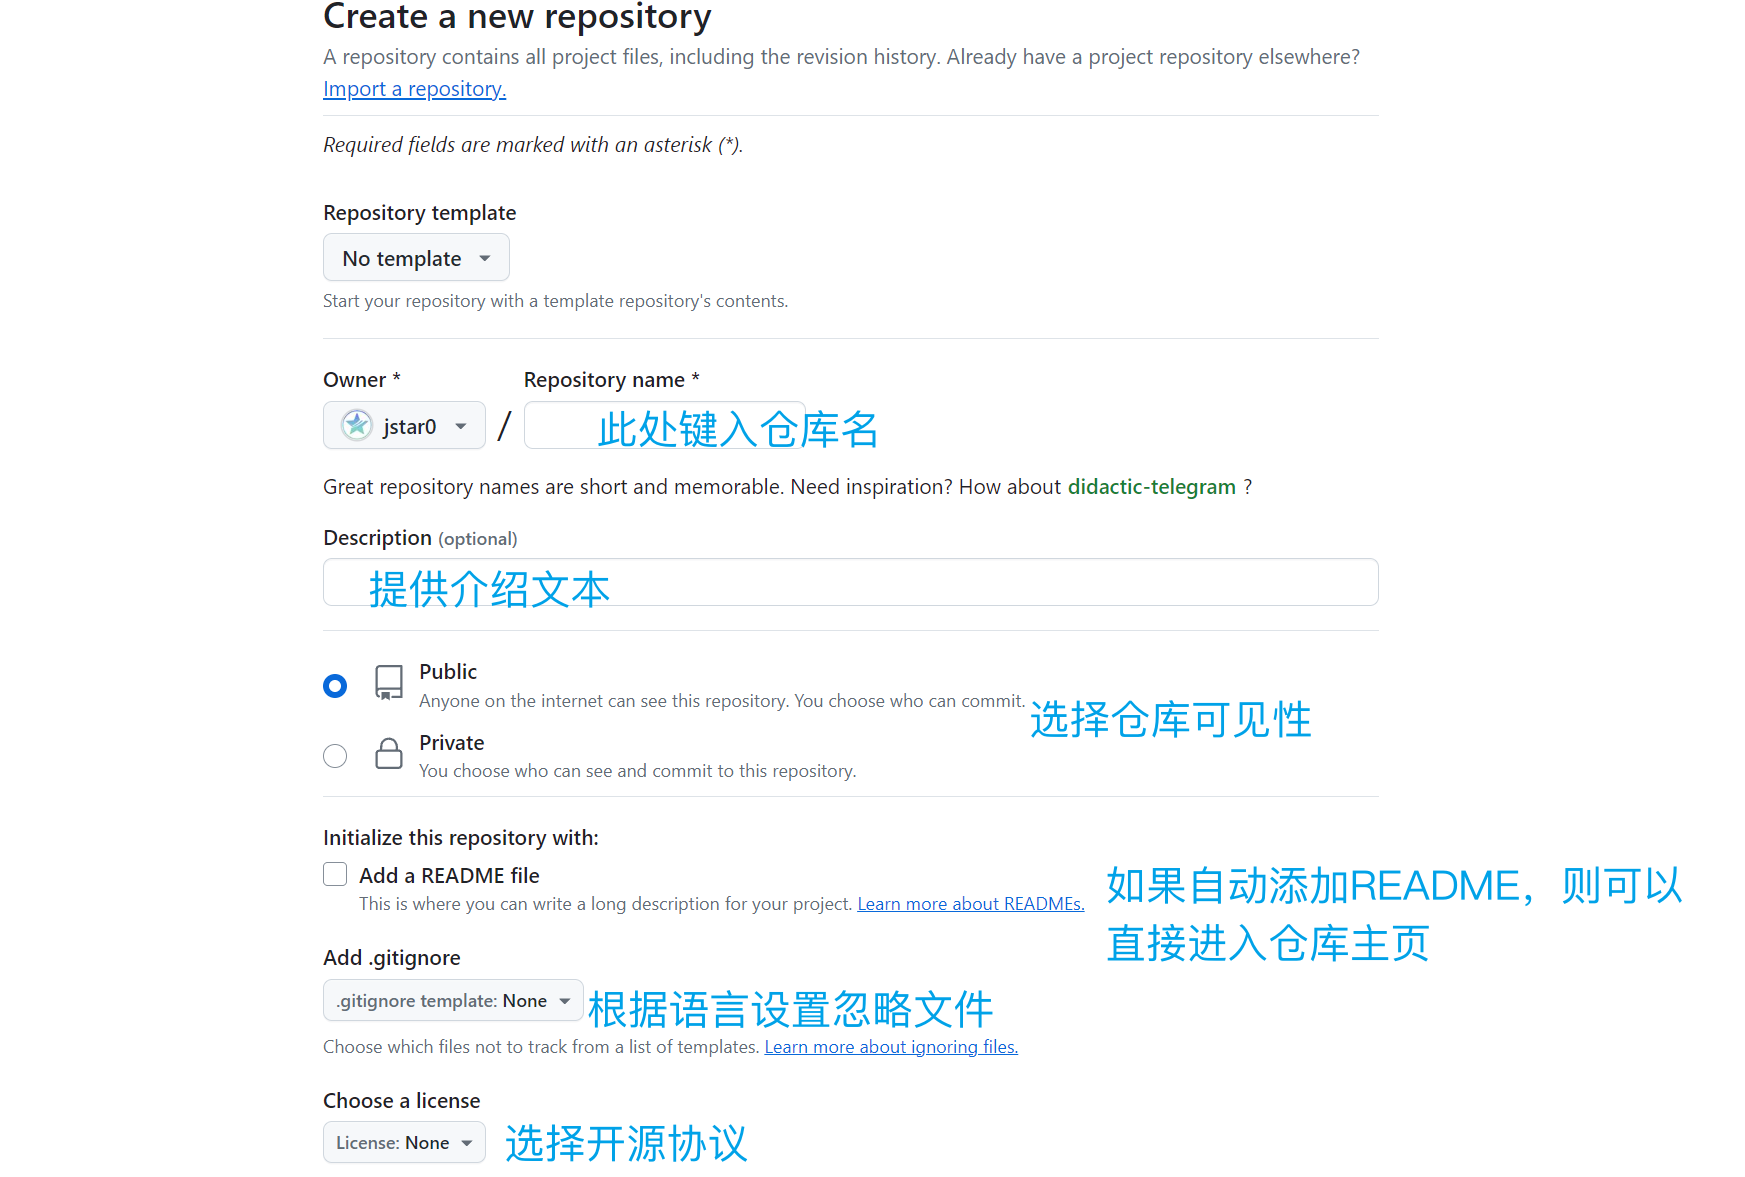
\includegraphics[width=0.65\textwidth]{figures/github-create-repo.png}
    \caption{在GitHub上创建一个仓库}
    \label{fig:github-create-repo}
\end{figure}

然后,我们可以使用\verb|git clone|命令将仓库克隆到本地:

\begin{listing}[!htpb]
    \begin{minted}{bash}
        git clone <url>
    \end{minted}
    \caption{CLONE(克隆)一个Git仓库}
\end{listing}

\subsection{添加、提交和查看}

在仓库中,最基本的操作就是,\textit{添加文件、提交文件,以及查看当前状态}。添加文件会将文件添加到\textbf{暂存区},而提交文件会将暂存区的文件提交到\textbf{版本库}。添加文件的操作如下:

\begin{listing}[!htpb]
    \begin{minted}{bash}
        git add <file>
    \end{minted}
    \caption{ADD(添加)文件到暂存区}
\end{listing}

如需提交所有文件,可以使用\texttt{*}(通配符),或者在不使用此指令而是使用\texttt{git commit -a}命令。但注意,使用此指令或许会造成不希望的结果。提交文件的操作如下:

\begin{listing}[!htpb]
    \begin{minted}{bash}
        git commit -m <message>
    \end{minted}
    \caption{COMMIT(提交)文件到版本库}
\end{listing}

注意,上述指令中\texttt{-m}参数可以留空,不过后期会自动打开一个文件要求输入Commit信息。查看当前状态的操作如下:

\begin{listing}[!htpb]
    \begin{minted}{bash}
        git status
    \end{minted}
    \caption{STATUS(状态)查看当前状态}
\end{listing}

上述操作是Git中最基本的操作,我们在本地创建一个仓库作为示例,如下图:

\begin{figure}[!h]
    \centering
    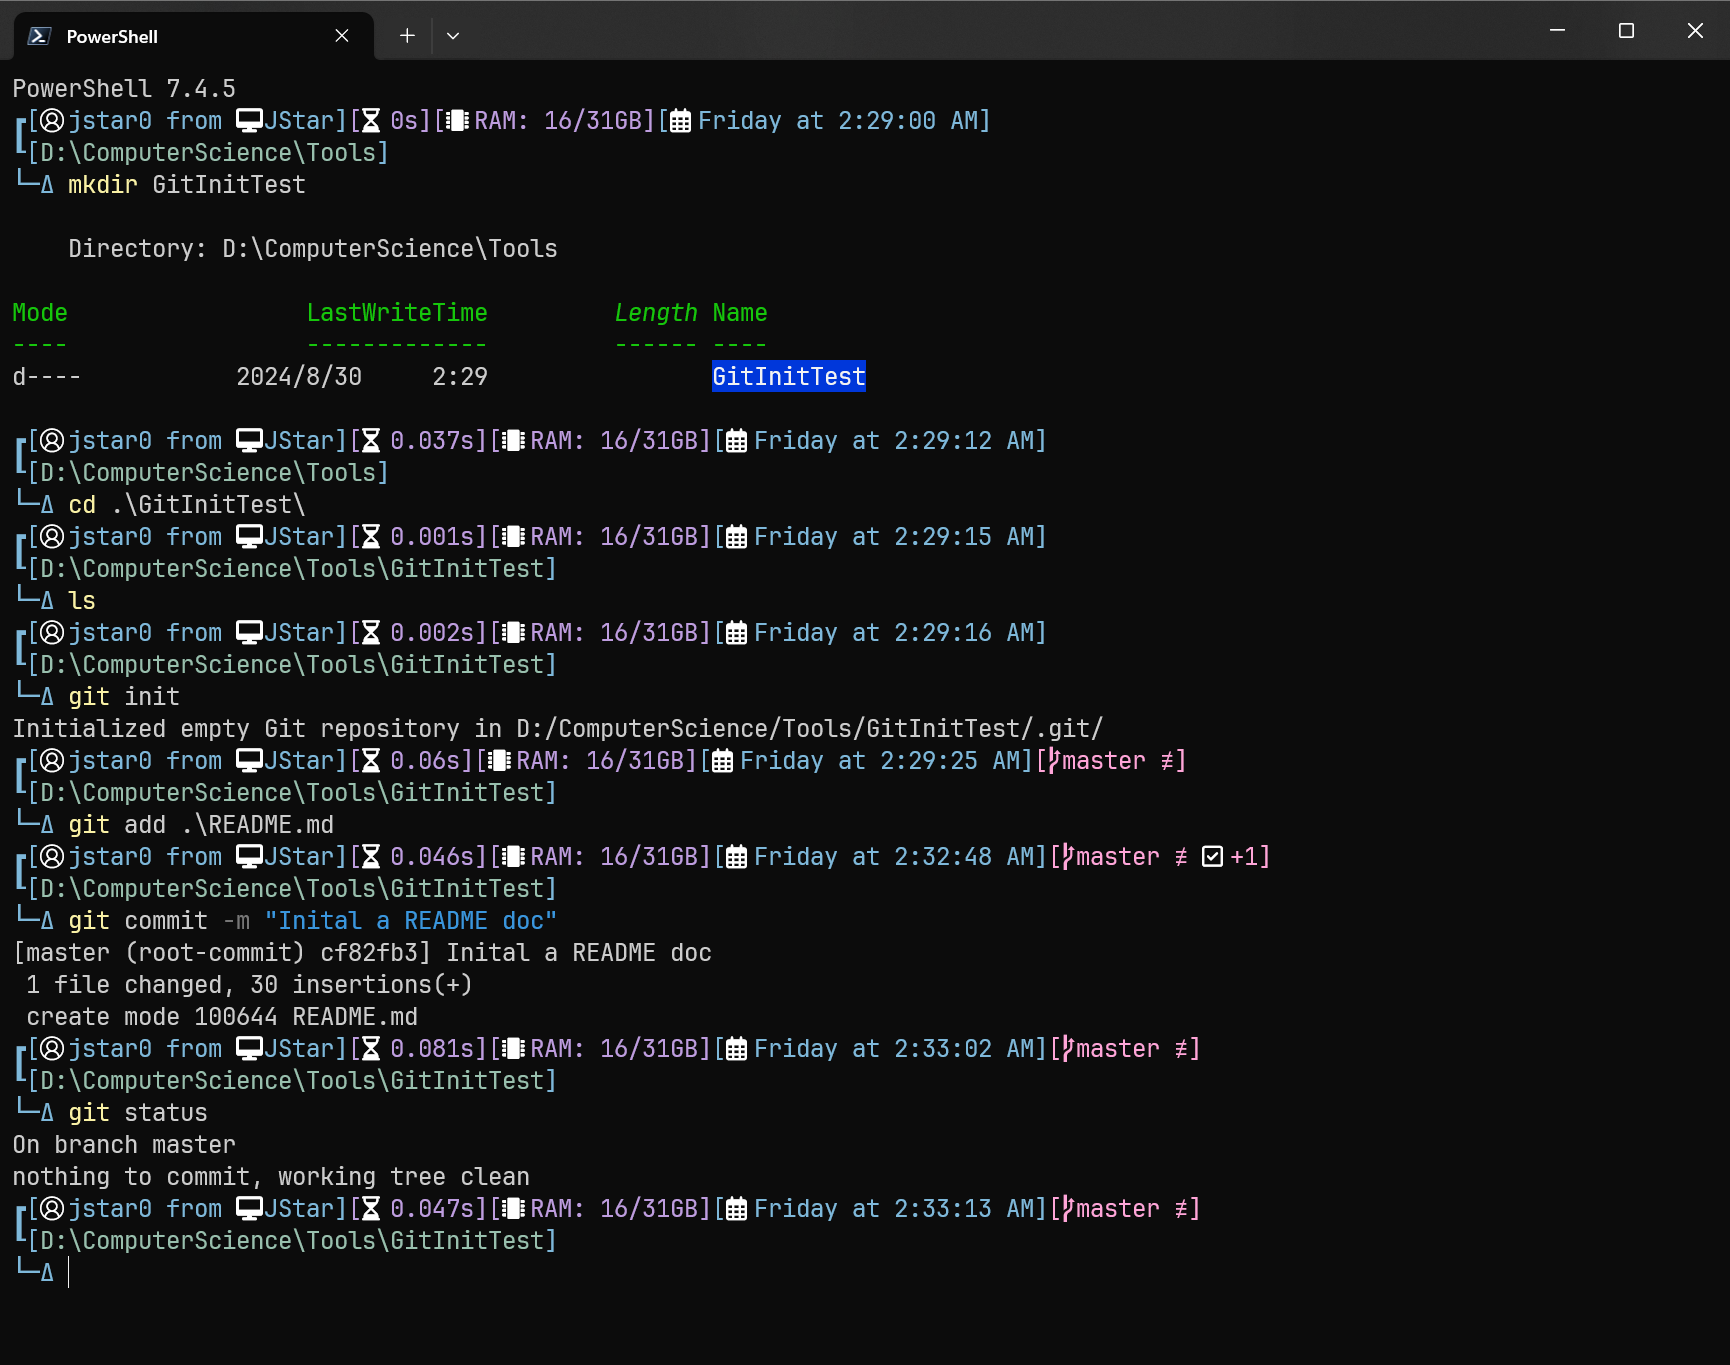
\includegraphics[width=0.65\textwidth]{figures/git-local-operations.png}
    \caption{本地操作创建、提交示例}
    \label{fig:git-local-operations}
\end{figure}

\subsection{推送到远端、拉取最新版本}

在本地操作完成后,我们可以将本地的提交推送到远程仓库,或者从远程仓库拉取最新版本。推送的操作如下: